%!TEX root = ../thesis.tex

%%%%%%%%%%%%%%%%%%%%%%%%%%%%%%%%%%%%%%%%%%%%%%%%%%%%%%
%%%%%%%%%%%%%%%%%%%%%%%%%%%%%%%%%%%%%%%%%%%%%%%%%%%%%%
\subsection{SAJaS}

\begin{frame}{SAJaS}
	Ações dos agentes são encapsuladas em ``Behaviours''
	
	Duas possibilidades de execução de implementação da comunicação:
	\begin{figure}[!h]
	\centering
		\begin{tikzpicture}
			\pause
			\node (img1) {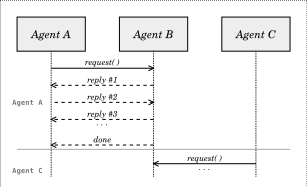
\includegraphics[height=4cm] {../figures/executionProblem.pdf}};
			\node (text1) at (img1.south) [yshift=-0.2cm] {(a) Acesso direto};
			\pause
			\node (img2) {\includegraphics[height=4cm]{../figures/executionProblem2.pdf}};
			\node (text1) at (img2.south) [yshift=-0.2cm] {
				\colorbox{white}{(b) Comunicação assíncrona}};
		\end{tikzpicture}
	\end{figure}

\end{frame}
\begin{frame}{SAJaS}
	Solução para comunicação ``assíncrona'' no SAJaS
	\begin{figure}
		\centering
		\begin{tikzpicture}
			\pause
			\node (img1) {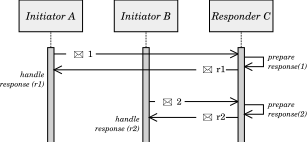
\includegraphics[height=3cm]
				{../figures/tickExample2.pdf}};
			\node (text1) at (img1.south) [yshift=-0.2cm] {JADE};
			\pause
			\node (img2) {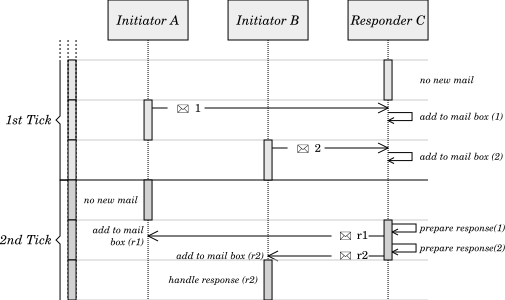
\includegraphics[height=6cm]
				{../figures/tickExample.pdf}};
			\node (text1) at (img2.south) [yshift=-0.2cm] {
				\colorbox{white}{SAJaS}};
		\end{tikzpicture}
	\end{figure}

\end{frame}

\subsection{Arquitetura}
\begin{frame}{Arquitetura}
	\begin{figure}
		\centering
		\begin{tikzpicture}
			\node (img1) {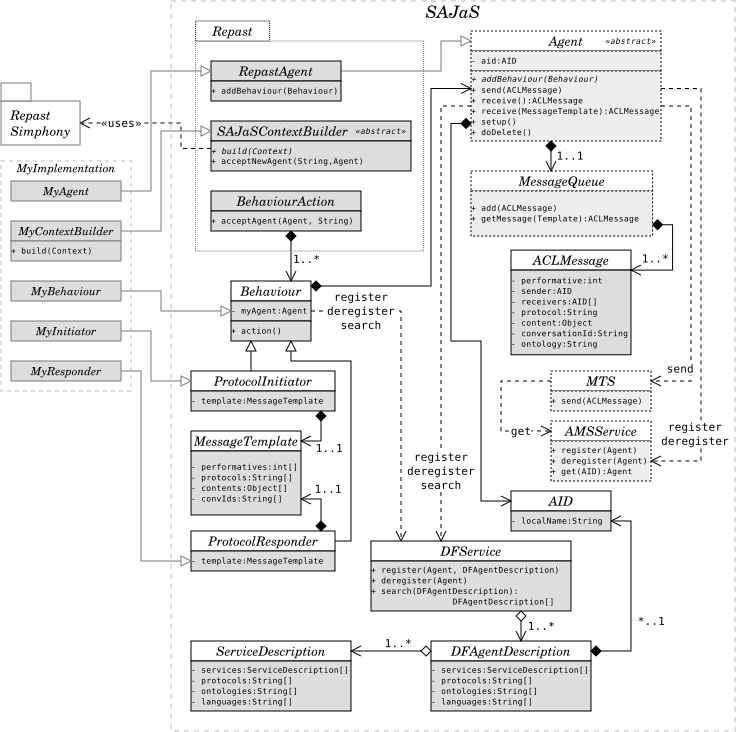
\includegraphics[height=6cm]
				{../figures/sajas_arch.pdf}};
			\node (text1) at (img1.south) [yshift=-0.2cm] {Arquitetura do SAJaS};
			\pause
			\node (img2) {\includegraphics[height=6cm]
				{figures/sajas_arch_simple.pdf}};
			\node (text1) at (img2.south) [yshift=-0.2cm] {
				\colorbox{white}{Arquitetura simplificada do SAJaS}};
		\end{tikzpicture}
	\end{figure}
\end{frame}

\subsection{FIPA}
\begin{frame}{FIPA}
	\begin{figure}
	\centering
	\includegraphics[width=0.7\linewidth]{../figures/sajas_arch_proto_simple.pdf}
	\caption[Behaviours and protocols in SAJaS]
	{Behaviours e Protocolos no SAJaS}
	\label{fig:arch_proto}
\end{figure}
\end{frame}